\documentclass[12]{article}
\usepackage{listings}

\usepackage{amsmath}
%\usepackage{datetime}
\usepackage{graphicx}
%\usepackage{times}
\usepackage{algorithm}

\usepackage{geometry}
\geometry{
  a4paper,
  total={210mm,297mm},
  left=20mm,
  right=20mm,
  top=20mm,
  bottom=20mm,
}


\title{\textbf{CSCI 6550 – Intelligent Agents\\Spring'23}\\\textbf{Homework-1}}
\author{Sharmin Aktar, 2581728}


\begin{document}

\begin{figure}
\centering

\includegraphics[width=0.5\textwidth]{images/uno_logo.png}
\end{figure}

\maketitle

\section*{Question and Answer}

\subsection*{Question 1}
What does the following expression mean?
\begin{center}
    $f: \mathbb{R}^2 \rightarrow \mathbb{R}$
\end{center}

\subsection*{Answer}
The above expression represents a mathematical function $f$ that maps two-dimensional real number into a single real number (scalar). For example, the function takes a pair of real numbers (x, y) and returns a corresponding real number scalar output based on the function design.

\subsection*{Question 2}
Write a function definition of above function in C++/Java.
\subsection*{Answer}

\begin{lstlisting}[language=Java]
public class myFunction {
  public static double func(double x, double y) {
        return x+y;
    }
  
  
  public static void main(String[] args) { 
    double x = 5.0;
    double y = 5.0;
    double output = func(x, y);
    System.out.println("Result:" + output);
  }
}
\end{lstlisting}




\subsection*{Question 3}
Suppose you are given the below two sets:

\begin{figure}
\centering
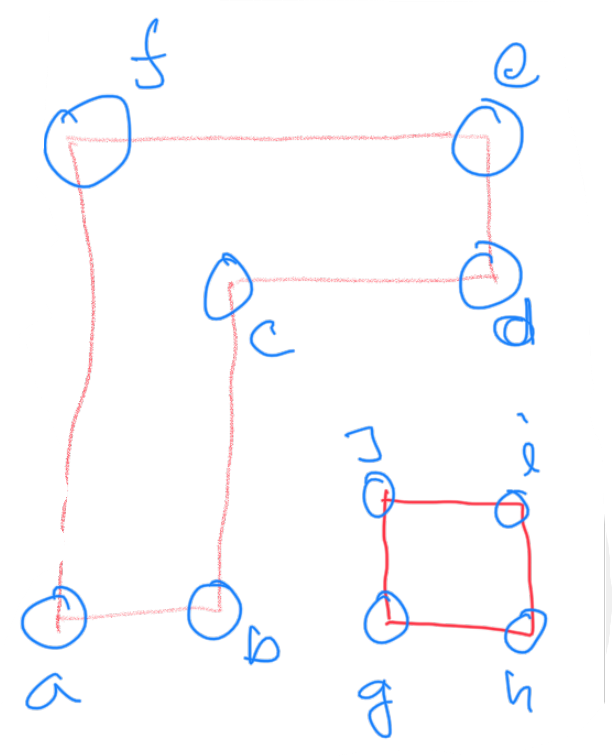
\includegraphics[width=0.3\textwidth]{images/set.png}
\end{figure}

\begin{center}
    A =\{a,b,c,d,e,f\}\\
    B=\{g,h,i,j\}
\end{center}

What is the name of the following set?
\begin{center}
C=\{A,B\}
\end{center}


\subsection*{Answer}

In mathematics, if two sets have no common elements, they are called disjoint sets. This can be stated as the intersection of two disjoint sets is an empty set. In the above example, A and B don't have any common elements, that's why they are disjoint. So, the set, C is considered as a set of disjoint sets or a group of disjoint sets.


\subsection*{Question 4}
Let $P(A)$ be the probability of event A to be happened and $P(B)$ be the probability of event B to be happened. \\ How to compute $P(B|A)$

\subsection*{Answer}

\begin{figure}[h]
\centering
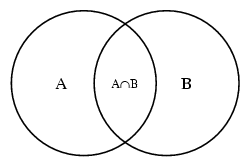
\includegraphics[width=0.3\textwidth]{images/venntwo.png}
\caption{Figure of 2 dependent set \cite{1}}
\end{figure}

If events A and B are dependent with each other, then the probability of the intersection of A and B (the probability that both events occur) is defined by the below equation \cite{2}:

\begin{equation}
P(A \cap B)=P(B|A)P(A) 
\label{eqn1}
\end{equation}
From the definition \ref{eqn1}, we can obtain the conditional probability $P(B|A)$  by dividing $P(A \cap B)$ with $P(A)$:

\begin{equation}
P(B|A)=\frac{P(A \cap B)}{P(A)}
\label{eqn2}
\end{equation}
 

\subsection*{Question 5}
 If A = TRUE, B=TRUE, C = FALSE then compute the following expression.\\
\begin{center}
   $\neg ( A \vee (B \land C) ) $ 
\end{center} 
\subsection*{Answer}
Here, A = TRUE, B=TRUE, C = FALSE \\
We know, Both relations must be true for the complex expression to be true in the logical relation AND($\land$).
If either relation is true, the complex expression is true in the logical relation OR ($\vee$) \cite{3}.

By using the rule, we can compute the above expression as below:\\
\begin{center}
$\neg ( A \vee (B \land C) ) $ \\
\implies $\neg ( TRUE \vee (TRUE \land FALSE )) $ \\
     \implies $\neg (TRUE \vee  FALSE)  $ \\
     \implies$\neg (TRUE)  $ \\
     \implies $FALSE$
      
     
\end{center}



\subsection*{Question 6}
What is the difference between tree and a graph?
\subsection*{Answer}

Trees and graphs are two important data structures used for representing connections between elements as a network of nodes and edges, but they have some key differences:

A Tree must contain the below characteristics:

\begin{itemize}
    \item having a specific root node
    \item must be connected without cycles
    \item must contain a unique path from the root to any other node
\end{itemize}
 
Whereas, Graphs have no such restrictions and can have cycles and multiple disconnected components. 

\subsection*{Question 7}
What is the computation complexity of searching a binary tree?
\subsection*{Answer}
The computation complexity of searching a binary tree is determined by its height and the number of nodes. On average, the time complexity of searching a binary tree is O(log n), 

\subsection*{Question 8}
What does the term "Topologically equivalent" mean? Give an example.

\subsection*{Answer}
The term "topologically equivalent" is used to describe the mathematical objects containing the same arrangement or configuration, which can be converted into each other through smooth changes, such as stretching or bending, without being cut or joined. 
For example, a circle and an ellipse can be considered topologically equivalent because they can be transformed into each other by altering their shape while still retaining their general structure. Conversely, a circle and a paper sheet are not topologically equivalent since they cant be transformed into each other without cutting or gluing. 

\subsection*{Question 9}
What is the Finite State Machine? Give an example.
\subsection*{Answer}

A Finite State Machine (FSM) is a mathematical model used to design systems with a finite number of states, which operates by receiving inputs and transitioning from one state to another based on these inputs. Each state in the FSM represents possible inputs, actions, and the subsequent state.

An example of a finite state machine is a traffic light which has three defined states, red, yellow, and green. It transitions between these states based on inputs (time). For instance, the traffic light switches from green to yellow when a set amount of time has passed. The transition from one state to another is controlled by the programming of the traffic light and is activated by the input of time elapsed.

\subsection*{Question 10}
What is the difference between feasible solution and optimal solution?

\subsection*{Answer}

A feasible solution is a solution that meets the requirements, while an optimal solution is the best feasible solution, providing the best outcome for an optimization problem. To summarize, we can say that, all optimal solutions are feasible solutions, but not all feasible solutions are optimal solutions. 

\begin{thebibliography}{9}
\bibitem{1} \href{http://www.biovenn.nl/venndiagram.tk/theory.html}
\bibitem{2} \href{http://www.stat.yale.edu/Courses/1997-98/101/condprob.htm}
\bibitem{3}\href{https://www.ibm.com/docs/en/spss-statistics/saas?topic=expressions-logical-operators}

\end{thebibliography}
\end{document}
